Im Folgenden sind die während des Versuchs aufgenommenen Messwert 
und die aus diesen berechneten Größen tabellarisch aufgeführt.
An entsprechender Stelle sind Erklärungen zu den Rechnungen und
Messwerten gegeben. Die Gleichungen zur Berechnung der angegebenen
Fehler sind Aufgrund ihrer hohen Komplexität nicht angegeben.     

\subsection{Messung des Frequenzverhältnisses}\label{sec:Auswertung_FrequenzVerhältnis}

	Die durch Abzählen bestimmte Anzahl der Schwingungamplituden $A_{1}$ pro 
	Schwebungsamplitude, das entsprechende Verhältnis sind in 
	\cref{tab:Schwebung} mit der jeweiligen Kapazität eingetragen dargestellt.  
	
	\begin{table}[!h]
	\centering
	\begin{tabular}{|c|c|c|c|c|c|c|}
		\hline
 		Gang & \multicolumn{3}{c|}{Frequenzdifferenz hin} & \multicolumn{3}{c|}{Frequenzdifferenz zurück} \\
		$g$ & $\Delta\nu_{h1}\,[\si{\hertz}]$ & $\Delta\nu_{h2}\,[\si{\hertz}]$ & $\left<\Delta\nu_{h}\right>\,[\si{\hertz}]$ & $\Delta\nu_{r1}\,[\si{\hertz}]$ & $\Delta\nu_{r2}\,[\si{\hertz}]$ & $\left<\Delta\nu_{r}\right>\,[\si{\hertz}]$\\\hline\hline
		\num{6}  & -  & -  & -  & -  & -  & - \\
		\num{12}  & \num{4(1)}  & \num{4(1)}  & \num{4.0(7)}  & \num{-11(1)}  & \num{-12(1)}  & \num{-11.5(7)} \\
		\num{18}  & \num{14(1)}  & \num{14(1)}  & \num{14.0(7)}  & \num{-18(1)}  & \num{-18(1)}  & \num{-18.0(7)} \\
		\num{24}  & \num{17(1)}  & \num{18(1)}  & \num{17.5(7)}  & \num{-24(1)}  & \num{-23(1)}  & \num{-23.5(7)} \\
		\num{30}  & \num{16(1)}  & \num{14(1)}  & \num{15.0(7)}  & \num{-28(1)}  & \num{-29(1)}  & \num{-28.5(7)} \\
		\num{36}  & \num{20(1)}  & \num{19(1)}  & \num{19.5(7)}  & \num{-34(1)}  & \num{-34(1)}  & \num{-34.0(7)} \\
		\num{42}  & \num{28(1)}  & \num{24(1)}  & \num{26.0(7)}  & \num{-34(1)}  & \num{-35(1)}  & \num{-34.5(7)} \\
		\num{48}  & \num{33(1)}  & \num{32(1)}  & \num{32.5(7)}  & \num{-34(1)}  & \num{-33(1)}  & \num{-33.5(7)} \\
		\num{54}  & \num{35(1)}  & \num{36(1)}  & \num{35.5(7)}  & \num{-30(1)}  & \num{-28(1)}  & \num{-29.0(7)} \\
		\num{60}  & \num{39(1)}  & \num{56(1)}  & \num{47.5(7)}  & \num{-27(1)}  & \num{-23(1)}  & \num{-25.0(7)} \\
		\hline
	\end{tabular}
	\caption{Direkt gemessene Frequenzen des Wagens in den verschiedenen Gängen \label{tab:Auswertung_Frequenz_Schwebung}}
\end{table}
	
	Mit Hilfe von \cref{eq:f+} und \cref{eq:f-} können die Fundamentalfrequenzen
	$ \nu^{+}\, \text{und}\, \nu^{-}$ aus den gegebenen Größen
	\begin{subequations}
		\begin{empheq}{align}
			C &= \SI{0.79320(5)}{\nano\farad} \\
			C_{sp} &= \SI{0.028}{\nano\farad} \\
			L &= \SI{23.95(5)}{\milli\henry}
		\end{empheq}
	\end{subequations}
	bestimmt werden. Diese Frequenzen sind in \cref{tab:Fundamental_Freqs} zu finden,
	in der auch das jeweilige  Verhältnis $\tfrac{2(\nu^{-} - \nu^{+})}{\nu^{-} + \nu^{+}}$
	der Schwebungs- zur Schwingungsfrequenz eingetragen ist.
	
	\begin{table}[!h]
	\centering
	\begin{tabular}{|c|c|c|c|}
		\hline
		Kapazitäten & Fundamentalfrequenz & Fundamentalfrequenz & Frequenzverhältnis\\
		$C_{K}\,[\si{\nano\farad}]$ & $\nu^{+}\,[\si{\kilo\hertz}]$ & $\nu^{-}\,[\si{\kilo\hertz}]$ & $\tfrac{2(\nu^{-} - \nu^{+})}{\nu^{-} + \nu^{+}}$\\\hline\hline
		\num{1.00(3)}  & \num{35.88(4)}  & \num{56.3(5)}  & \num{0.442(8)} \\
		\num{2.19(7)}  & \num{35.88(4)}  & \num{46.6(3)}  & \num{0.259(6)} \\
		\num{2.86(9)}  & \num{35.88(4)}  & \num{44.3(2)}  & \num{0.210(5)} \\
		\num{4.7(1)}  & \num{35.88(4)}  & \num{41.2(2)}  & \num{0.138(4)} \\
		\num{6.9(2)}  & \num{35.88(4)}  & \num{39.7(1)}  & \num{0.100(3)} \\
		\num{8.2(2)}  & \num{35.88(4)}  & \num{39.1(1)}  & \num{0.085(2)} \\
		\num{10.0(3)}  & \num{35.88(4)}  & \num{38.52(9)}  & \num{0.071(2)} \\
		\num{12.0(4)}  & \num{35.88(4)}  & \num{38.10(8)}  & \num{0.060(2)} \\
		\hline
	\end{tabular}
	\caption{Berechnete Fundamentalfrequenzen und das Frequenzverhältnis der Schwebung \label{tab:Fundamental_Freqs}}
\end{table}
	
	Die relativen Abweichungen der gemessenen von den berechneten Werten des Frequenzverhältnisses
	$ N_{t} := \tfrac{2(\nu^{-} - \nu^{+})}{\nu^{-} + \nu^{+}}$ und $N_{m} := \tfrac{1}{A_{1}}$ sind in \cref{tab:FrequenzVerhältnis} enthalten.
	
	\input{Daten/Tabelle_FrequenzVerhältnis.tex}
\newpage	
\subsection{Messung der Fundamentalfrequenzen}\label{sec:Auswertung_FundamentalFrequenz}
	
	Die gemessenen Fundamentalfrequenzen der gekoppelten Schwingkreise
	sind in \cref{tab:Fundamental_Messung} zusammen mit den berechneten
	Fundamentalfrequenzen aus \cref{tab:Fundamental_Freqs}  zu finden.
	Neben diesen sind dort auch die Verhältnisse von gemessener zu 
	berechneter Frequenz angegeben. 
	
	\begin{table}[!h]
	\centering
	\begin{tabular}{|c|c|c|c|c|c|}
		\hline
%		Fundamentalfrequenz & Fundamentalfrequenz & Fundamentalfrequenz & Fundamentalfrequenz & Frequenzverhältnis & Frequenzverhältnis\\
		\multicolumn{2}{|c|}{Berechnete} & \multicolumn{2}{c|}{Gemessene} & \multicolumn{2}{c|}{ } \\
		\multicolumn{2}{|c|}{Fundamentalfrequenzen} & \multicolumn{2}{c|}{Fundamentalfrequenzen} &
		\multicolumn{2}{c|}{Frequenzverhältnis} \\
		$\nu^{+}_{theo}\,[\si{\kilo\hertz}]$ & $\nu^{-}_{theo}\,[\si{\kilo\hertz}]$ & $\nu^{+}\,[\si{\kilo\hertz}]$ & $\nu^{-}\,[\si{\kilo\hertz}]$ & $\sfrac{\nu^{+}}{\nu^{+}_{theo}}$ & $\sfrac{\nu^{-}}{\nu^{-}_{theo}}$\\\hline\hline
		\num{35.88(4)}  & \num{56.3(5)}  & \num{35.65(1)}  & \num{40.68(1)}  & \num{0.993(1)}  & \num{0.723(6)} \\
		\num{35.88(4)}  & \num{46.6(3)}  & \num{35.65(1)}  & \num{39.61(1)}  & \num{0.993(1)}  & \num{0.851(5)} \\
		\num{35.88(4)}  & \num{44.3(2)}  & \num{35.65(1)}  & \num{39.06(1)}  & \num{0.993(1)}  & \num{0.881(5)} \\
		\num{35.88(4)}  & \num{41.2(2)}  & \num{35.65(1)}  & \num{39.25(1)}  & \num{0.993(1)}  & \num{0.952(4)} \\
		\num{35.88(4)}  & \num{39.7(1)}  & \num{35.63(1)}  & \num{37.83(1)}  & \num{0.993(1)}  & \num{0.954(3)} \\
		\num{35.88(4)}  & \num{39.1(1)}  & \num{35.62(1)}  & \num{37.22(1)}  & \num{0.993(1)}  & \num{0.952(2)} \\
		\num{35.88(4)}  & \num{38.52(9)}  & \num{35.62(1)}  & \num{37.15(1)}  & \num{0.993(1)}  & \num{0.964(2)} \\
		\num{35.88(4)}  & \num{38.10(8)}  & \num{35.60(1)}  & \num{37.09(1)}  & \num{0.992(1)}  & \num{0.974(2)} \\
		\hline
	\end{tabular}
	\caption{Berechnete und gemessene Fundamentalfrequenzen mit jeweiligem Verhältnis \label{tab:Fundamental_Messung}}
\end{table}
	
	In \cref{fig:Auswertung_FundamentalKurven} sind die gemessenen Fundamentalfrequenzen $\nu^{+}\ \text{und}\ \nu^{-}$ 
	in Abhängigkeit von der Kapazität des Koppelkondensators $C_{K}$ zusammen mit dem theoretischen Verlauf dieser 
	Abhängigkeit aufgetragen.
	
	\begin{figure}[!h]
		\centering
		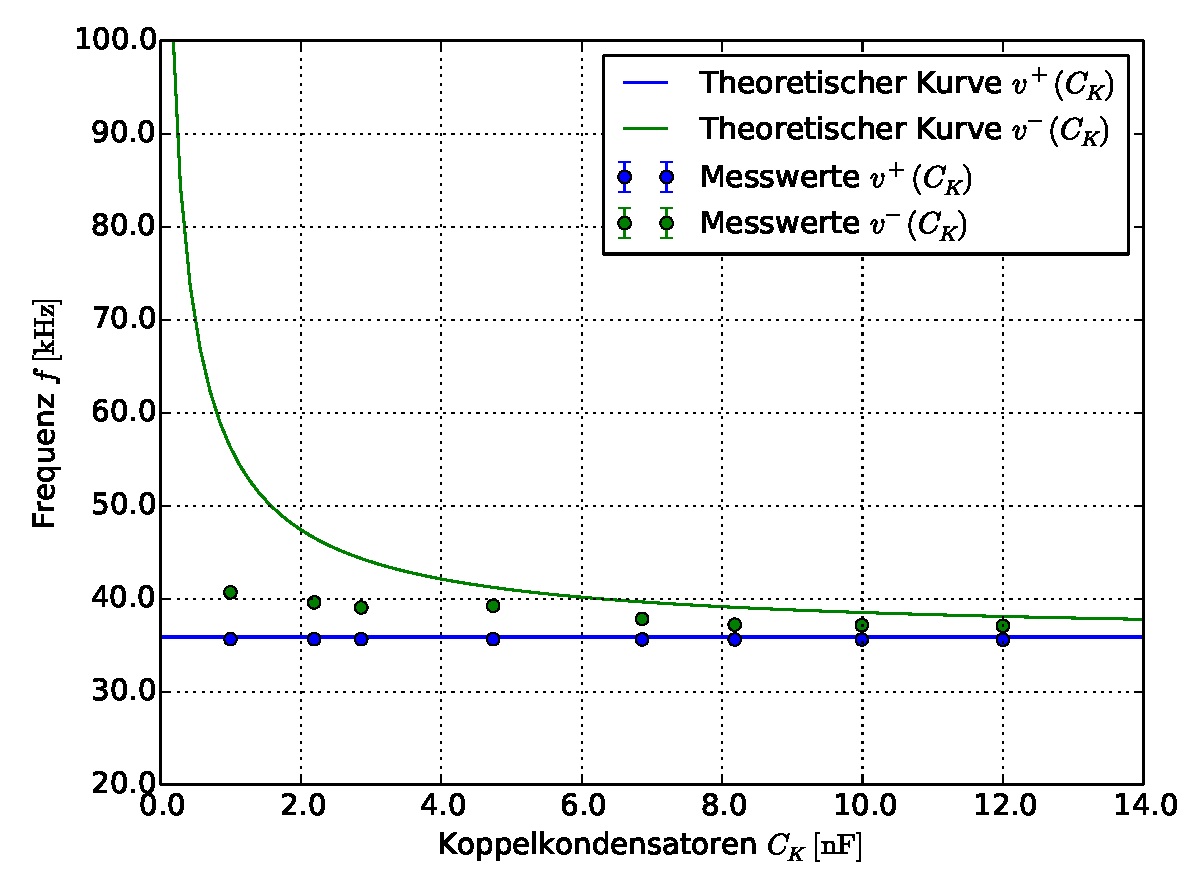
\includegraphics[scale=0.7]{Grafiken/Frequenz_CK.pdf}
		\caption{Darstellung der gemessenen Fundamentalfrequenzen und deren Theoriekurven}
		\label{fig:Auswertung_FundamentalKurven}
	\end{figure}  
	
	
\subsection{Messung des Verlaufs des Stroms $I_{2}$} \label{sec:Auswertung_Wobbel}
	
	Der auf dem Oszilloskop angezeigte Verlauf der Spannung in Abhängigkeit von der Frequenz, ist für jeden 
	Koppelkondensator $C_{K}$ ähnlich zu dem in \cref{fig:WobbelVerlauf} für den Kondensator mit 
	$C_{K} = \SI{2.19(7)}{\nano\farad}$ dargestellten.
	

	Die aus diesen Bildern bestimmten Messwerte für die Fundamentalfrequenzen und die zugehörigen Spannungen
	sind in \cref{tab:WobbelVerlauf} aufgeführt.  

	\begin{table}[!h]
	\centering
	\begin{tabular}{|c|c|c|c|c|}
		\hline
		Kapazitäten & Fundamentalfrequenz & Fundamentalfrequenz & Spannung & Spannung\\
		$C_{K}\,[\si{\nano\farad}]$ & $\nu^{+}\,[\si{\kilo\hertz}]$ & $\nu^{-}\,[\si{\kilo\hertz}]$ & $U^{+}\,[\si{\volt}]$ & $U^{-}\,[\si{\volt}]$\\\hline\hline
		\num{2.19(7)}  & \num{38.0(8)}  & \num{48.5(8)}  & \num{2.00(5)}  & \num{1.10(5)} \\
		\num{2.86(9)}  & \num{37.2(8)}  & \num{46.2(8)}  & \num{2.00(5)}  & \num{1.10(5)} \\
		\num{4.7(1)}  & \num{38.0(8)}  & \num{43.2(8)}  & \num{2.05(5)}  & \num{1.15(5)} \\
		\num{6.9(2)}  & \num{38.0(8)}  & \num{41.0(8)}  & \num{2.05(5)}  & \num{1.15(5)} \\
		\num{8.2(2)}  & \num{38.0(8)}  & \num{40.2(8)}  & \num{2.10(5)}  & \num{1.15(5)} \\
		\num{10.0(3)}  & \num{38.0(8)}  & \num{39.5(8)}  & \num{2.10(5)}  & \num{1.20(5)} \\
		\num{12.0(4)}  & \num{37.2(8)}  & \num{38.8(8)}  & \num{2.10(5)}  & \num{1.25(5)} \\
		\hline
	\end{tabular}
	\caption{Fundamentalfrequenzen und jeweilige Spannungsspitzen \label{tab:WobbelVerlauf}}
\end{table}
	
	Die zu untersuchende Stromstärke lässt sich aus den Spannungen in \cref{tab:WobbelVerlauf} mit Hilfe von
	\begin{empheq}{equation}
		I =  \dfrac{U}{R}
	\end{empheq}  
	berechnen. Zusammen mit den Mittels \cref{eq:I2} berechneten Werten für diese Stromstärke, sind diese in
	\cref{tab:I2} eingetragen. Für die Berechnung der Stromstärken, wurde die Generatorspannung $\envert{\mathfrak{U}} = \SI{4}{\volt}$ verwendet. 
	
	\begin{table}[!h]
	\centering
	\begin{tabular}{|c|c|c|c|}
		\hline
		\multicolumn{2}{|c}{Berechnet}& \multicolumn{2}{|c|}{Gemessen}\\
		Stromstärke & Stromstärke & Stromstärke & Stromstärke\\
		$I^{+}\,[\si{\ampere}]$ & $I^{-}\,[\si{\ampere}]$ & $I^{+}\,[\si{\ampere}]$ & $I^{-}\,[\si{\ampere}]$\\\hline\hline
		\num{0.005(2)}  & \num{0.01(1)}  & \num{0.0256(6)}  & \num{0.0141(6)} \\
		\num{0.009(8)}  & \num{0.008(8)}  & \num{0.0256(6)}  & \num{0.0141(6)} \\
		\num{0.006(2)}  & \num{0.005(4)}  & \num{0.0263(6)}  & \num{0.0147(6)} \\
		\num{0.007(1)}  & \num{0.01(1)}  & \num{0.0263(6)}  & \num{0.0147(6)} \\
		\num{0.0078(8)}  & \num{0.01(2)}  & \num{0.0269(6)}  & \num{0.0147(6)} \\
		\num{0.0092(7)}  & \num{0.02(3)}  & \num{0.0269(6)}  & \num{0.0154(6)} \\
		\num{0.012(5)}  & \num{0.02(2)}  & \num{0.0269(6)}  & \num{0.0160(6)} \\
		\hline
	\end{tabular}
	\caption{Theoretisch bestimmte und gemessene Stromstärken \label{tab:I2}}
\end{table}	
	
	\begin{figure}
			\centering
			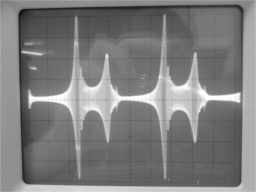
\includegraphics[scale=0.8]{Grafiken/Kondensator2.jpg}
			\caption{Beispielhafter Verlauf der Spannung für $C_{K} = \SI{2.19(7)}{\nano\farad}$ }
			\label{fig:WobbelVerlauf}
	\end{figure}
	
	Die in \cref{fig:C1} bis \ref{fig:C7} dargestellten Graphen zeigen den theoretischen Verlauf der Stromstärke nach 
	\cref{eq:I2}, für eine Auswahl der verwendeten Koppelkondensatoren.


%	\begin{figure}[!h]
%		\centering
%    	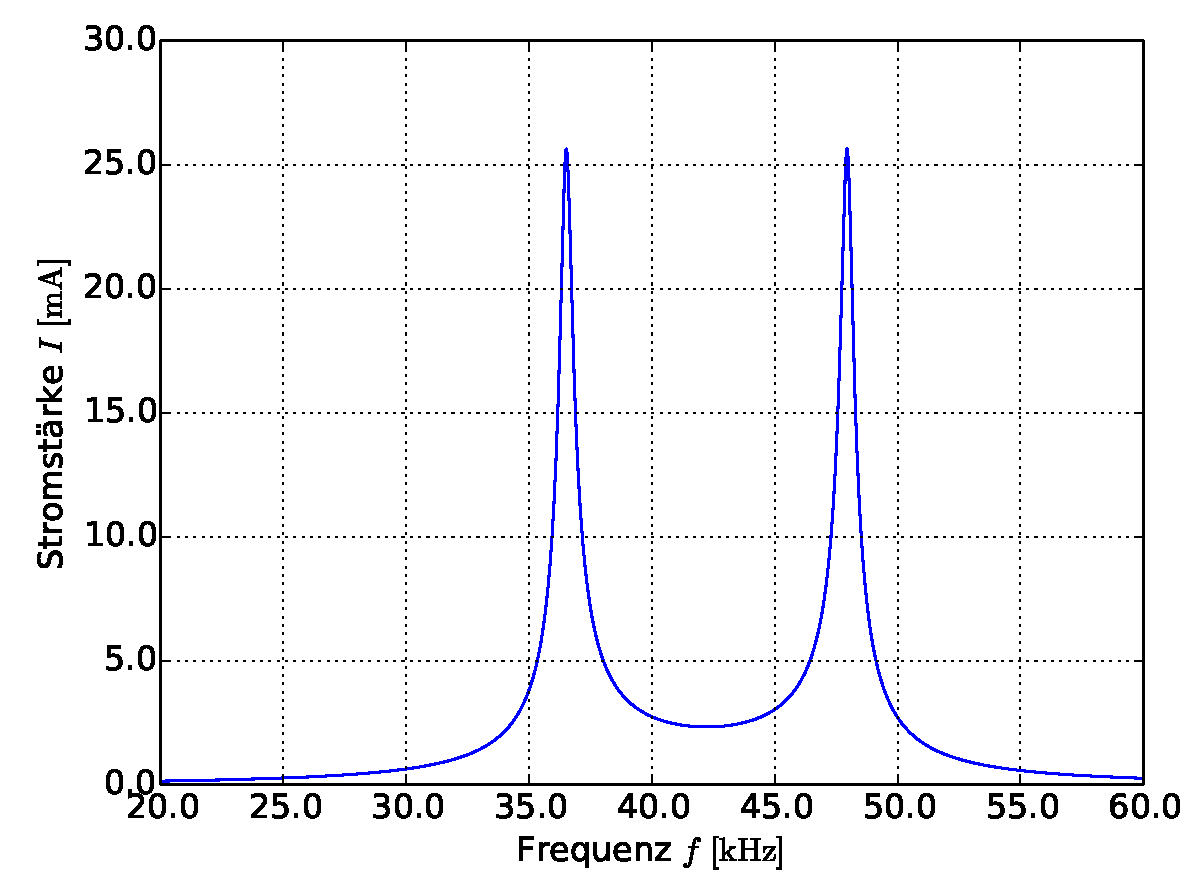
\includegraphics[scale=0.7]{Grafiken/Stromverlauf1.pdf}
%		\caption{Stromverläufe unter Verwendung von $C_{K} = \SI{2.19(7)}{\nano\farad}$}
%		\label{fig:C1} 
%	\end{figure}
%		
%	\begin{figure}[]
%		\centering
%    	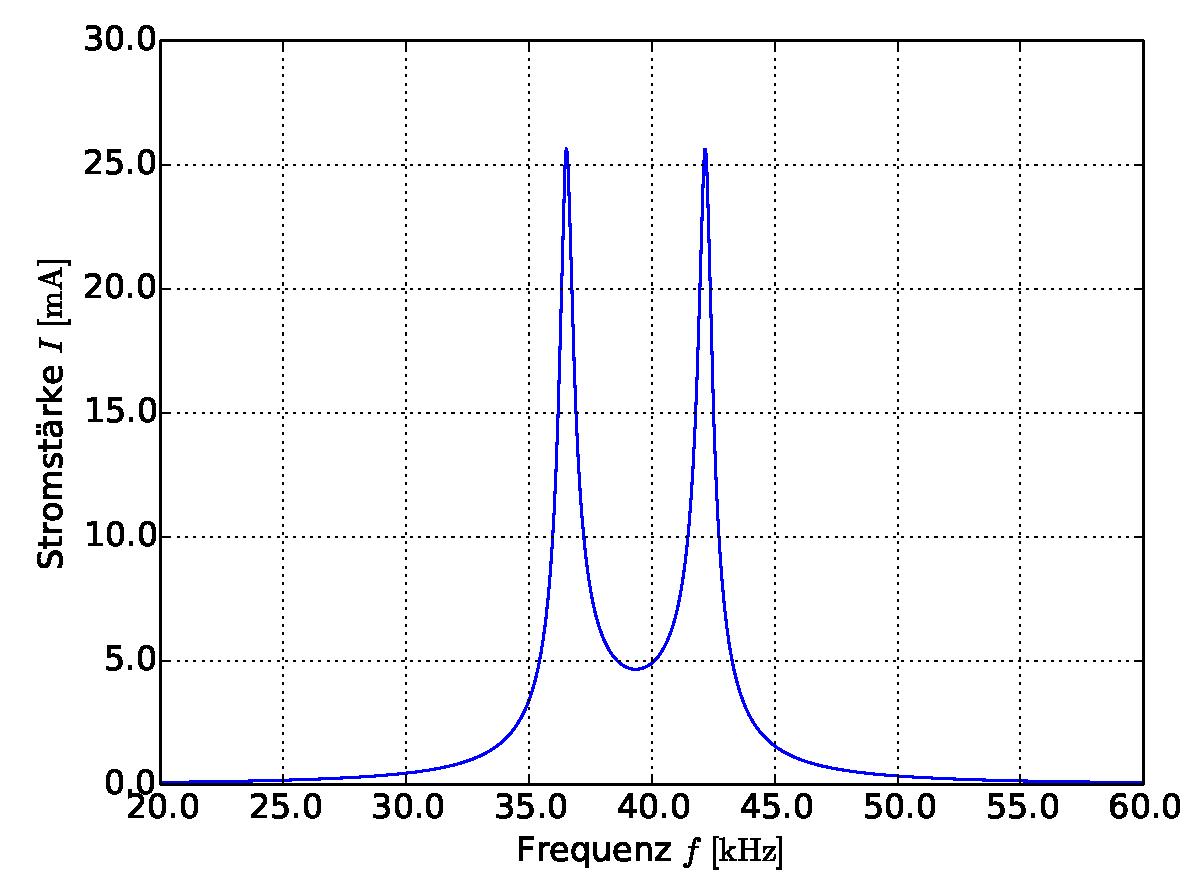
\includegraphics[scale=0.7]{Grafiken/Stromverlauf3.pdf}
%		\caption{Stromverläufe unter Verwendung von $C_{K} = \SI{4.7(1)}{\nano\farad}$}
%		\label{fig:C3} 
%	\end{figure}
%	
%	\begin{figure}[]
%		\centering
%    	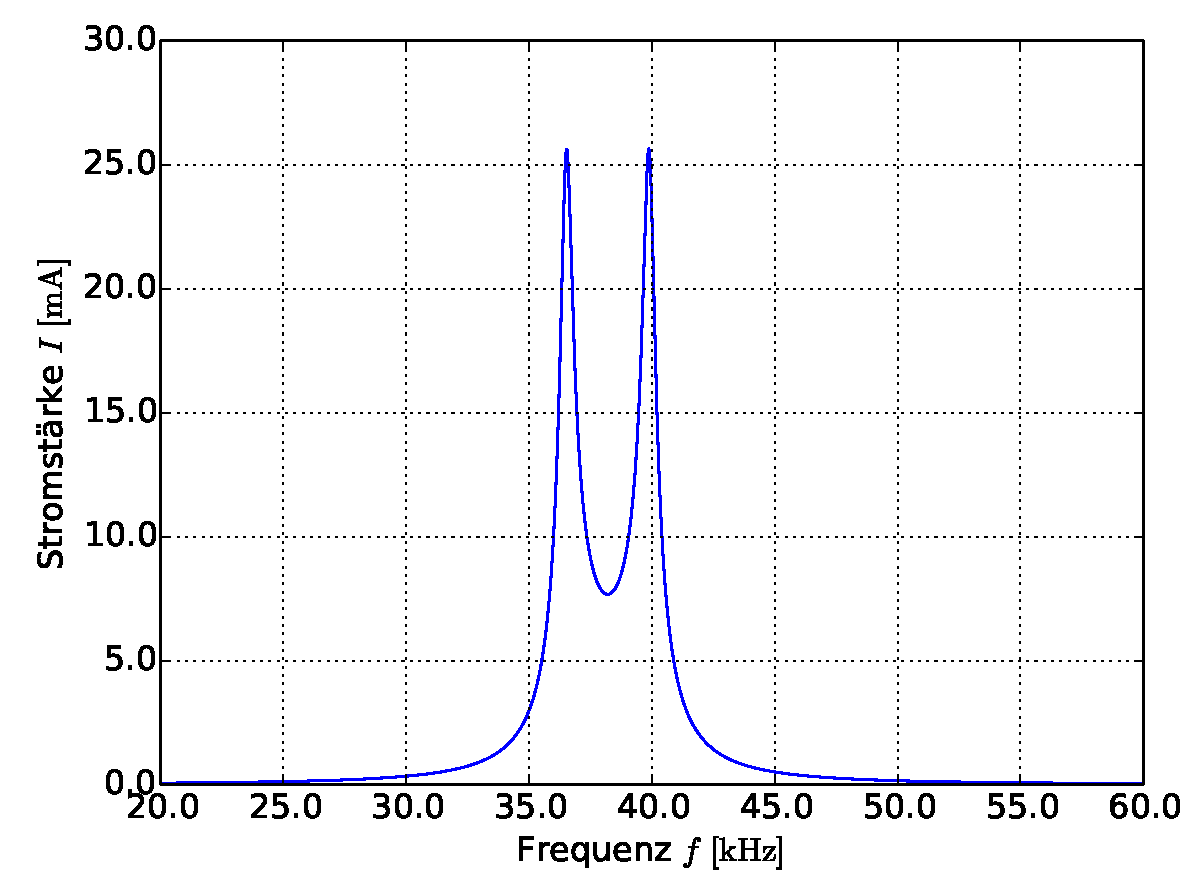
\includegraphics[scale=0.7]{Grafiken/Stromverlauf5.pdf}
%		\caption{Stromverläufe unter Verwendung von $C_{K} = \SI{8.2(2)}{\nano\farad}$}
%		\label{fig:C5} 
%	\end{figure}	
%	
%	\begin{figure}[]
%		\centering
%    	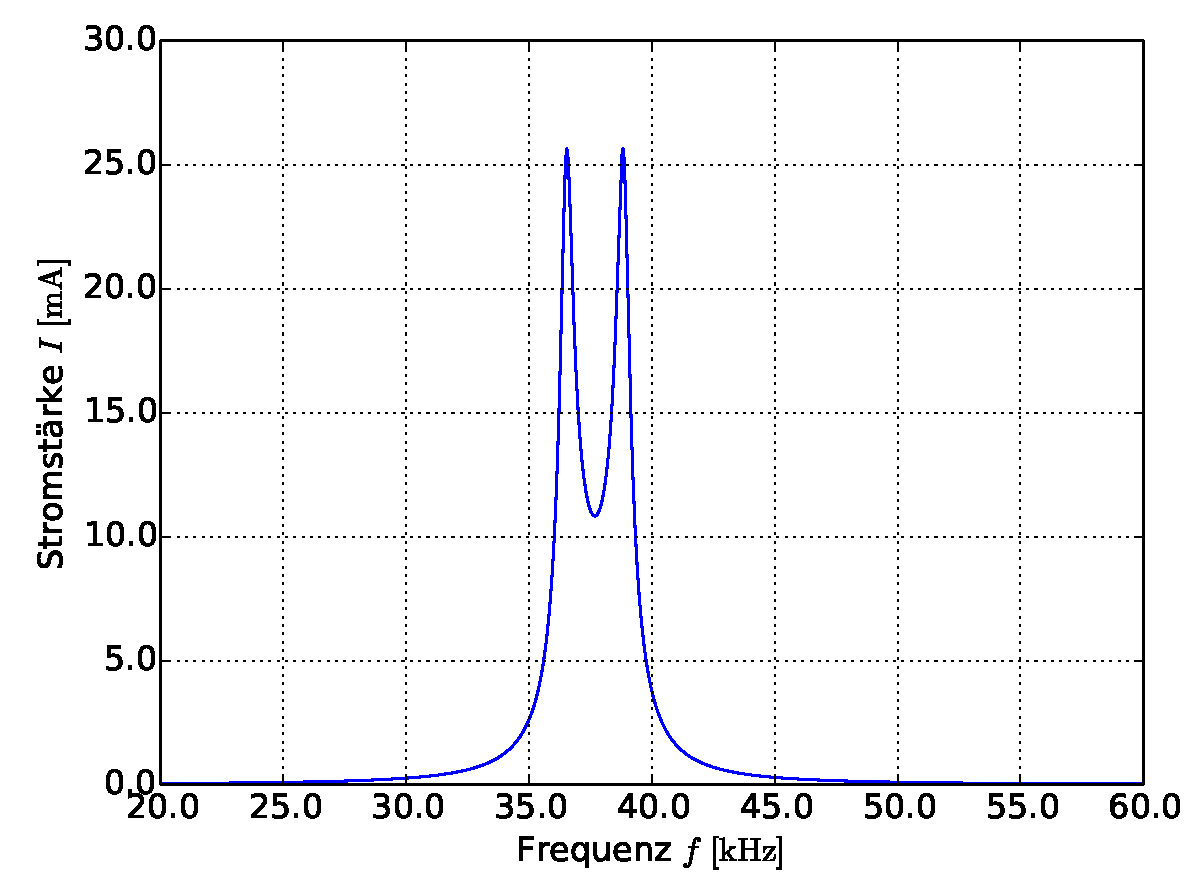
\includegraphics[scale=0.7]{Grafiken/Stromverlauf7.pdf}
%		\caption{Stromverläufe unter Verwendung von $C_{K} = \SI{12.0(4)}{\nano\farad}$}
%		\label{fig:C7} 
%	\end{figure}
		
\begin{figure}
		\subfloat[$C_{K} = \SI{2.19(7)}{\nano\farad}$\label{fig:C1}] {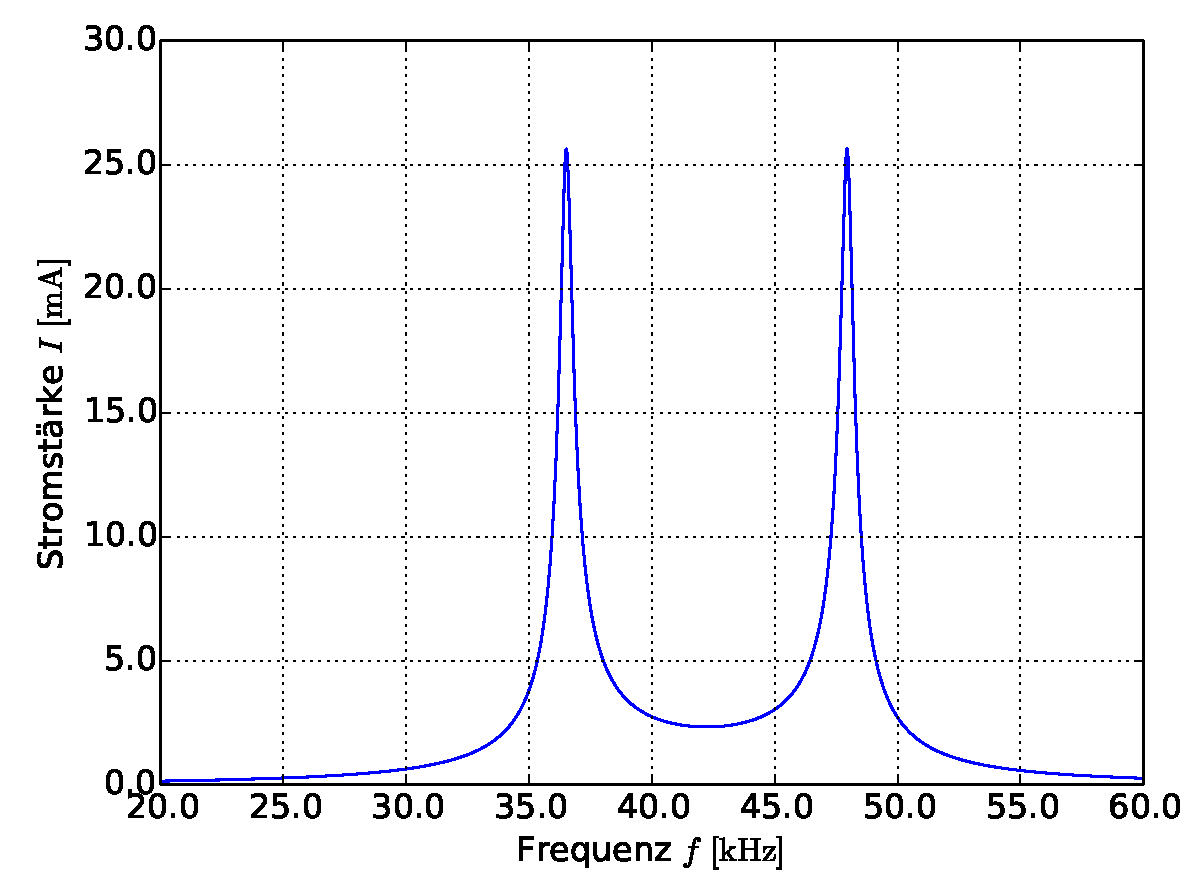
\includegraphics[scale=0.4]{Grafiken/Stromverlauf1.pdf}}
%		\subfloat[$C_{K} = \SI{2.19(7)}{\nano\farad}$\label{fig:C2}] {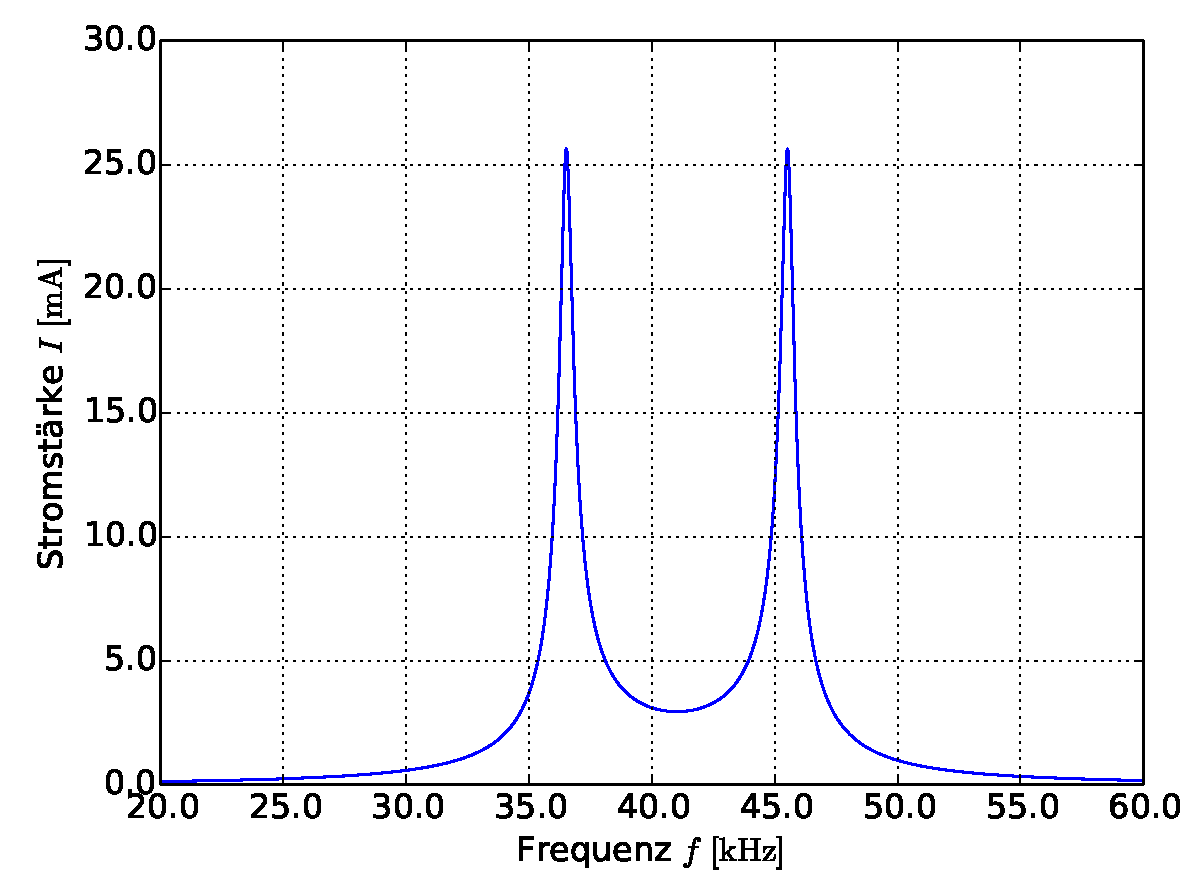
\includegraphics[scale=0.4]{Grafiken/Stromverlauf2.pdf}}\\
		\subfloat[$C_{K} = \SI{4.7(1)}{\nano\farad}$\label{fig:C3}] {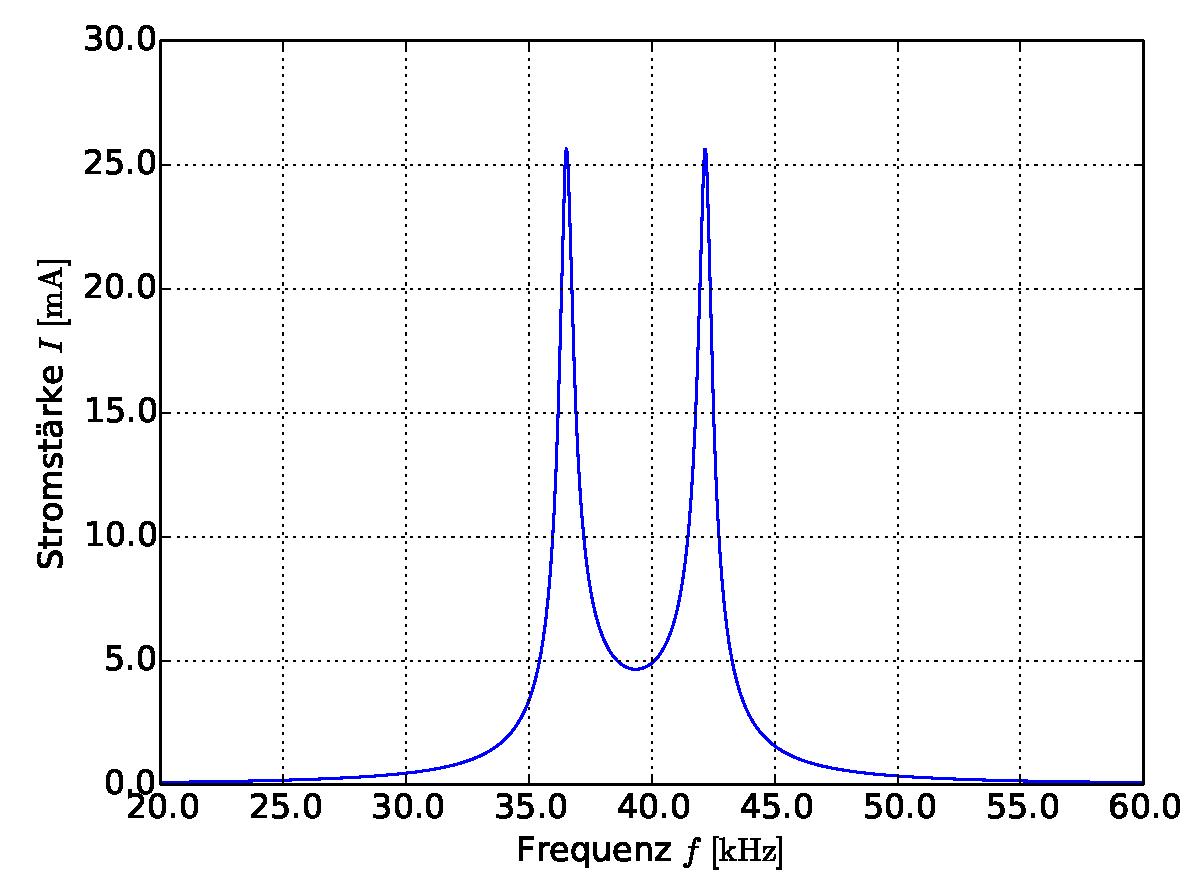
\includegraphics[scale=0.4]{Grafiken/Stromverlauf3.pdf}}\\
%		\subfloat[$C_{K} = \SI{8.2(2)}{\nano\farad}$\label{fig:C4}] {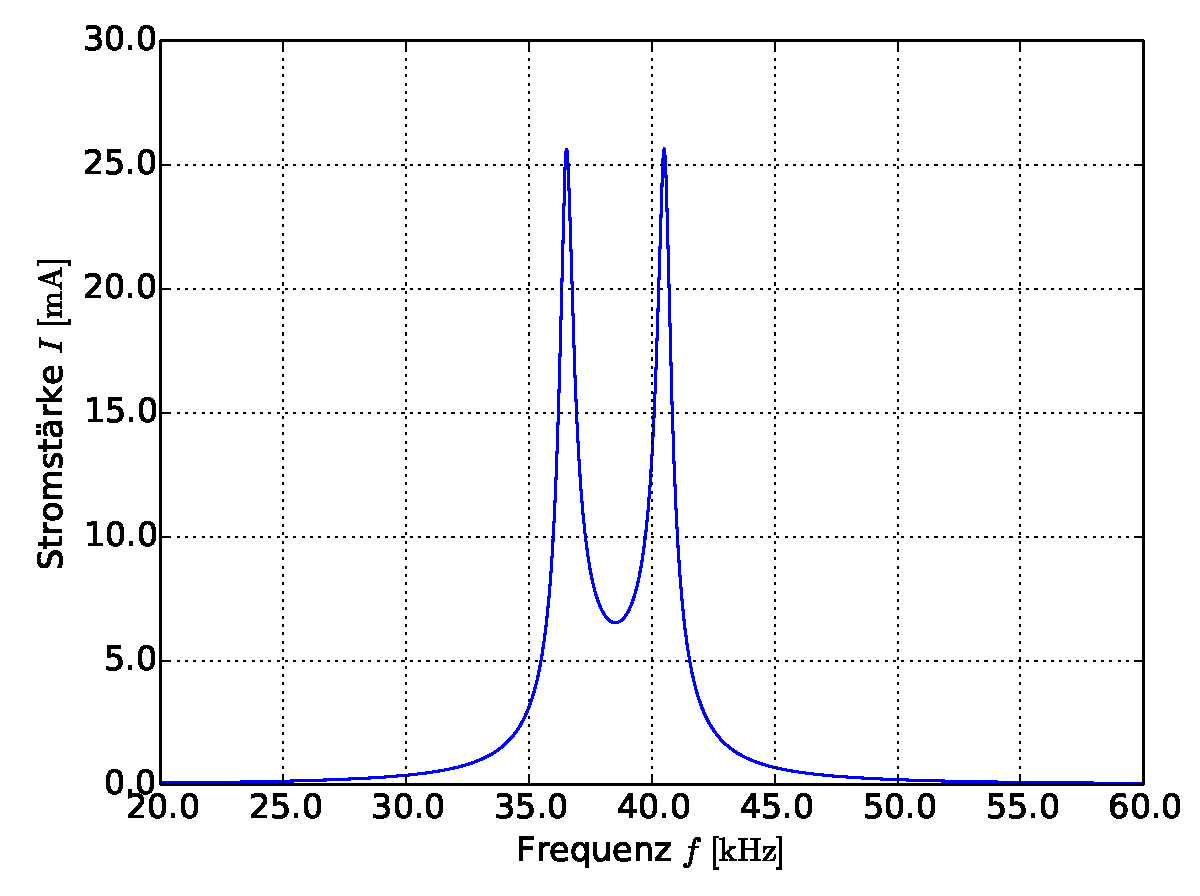
\includegraphics[scale=0.4]{Grafiken/Stromverlauf4.pdf}}\\
		\subfloat[$C_{K} = \SI{8.2(2)}{\nano\farad}$\label{fig:C5}] {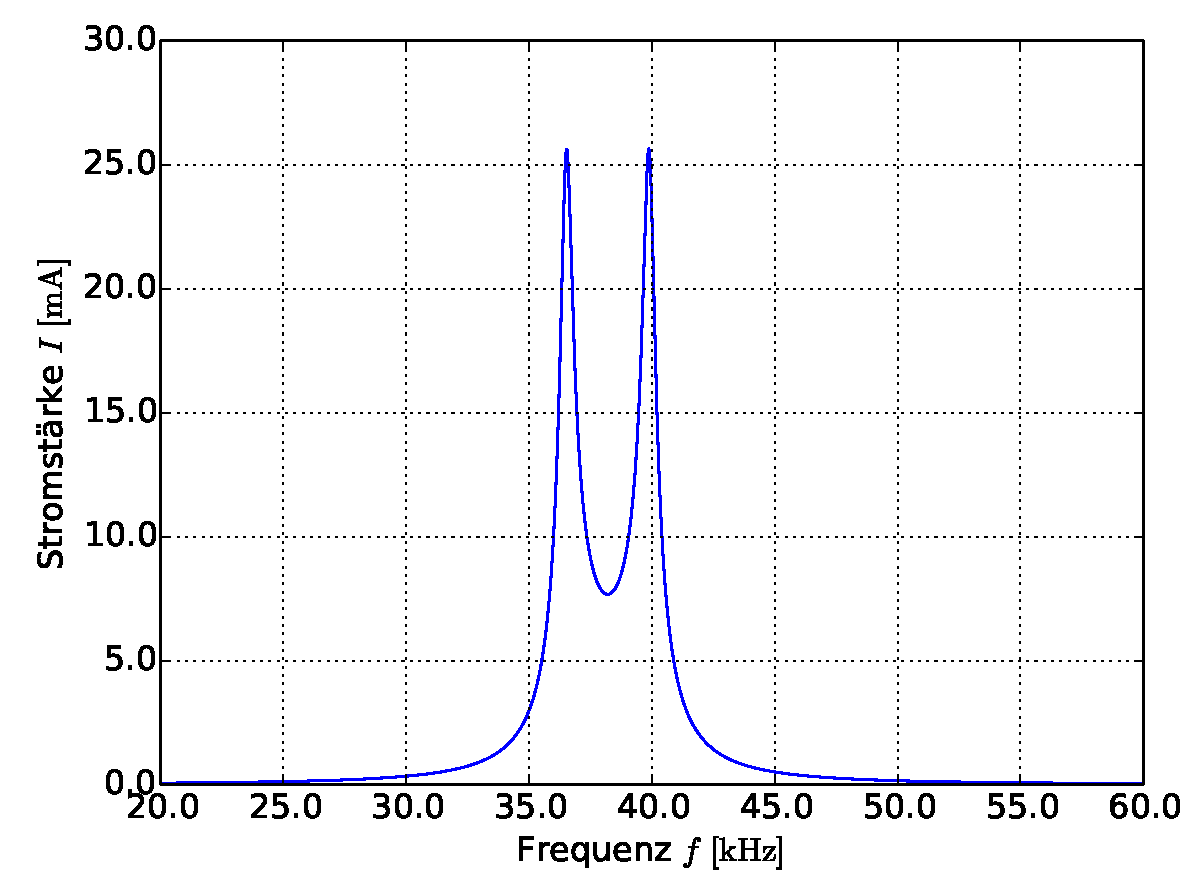
\includegraphics[scale=0.4]{Grafiken/Stromverlauf5.pdf}}
		\subfloat[$C_{K} = \SI{12.0(4)}{\nano\farad}$\label{fig:C7}] {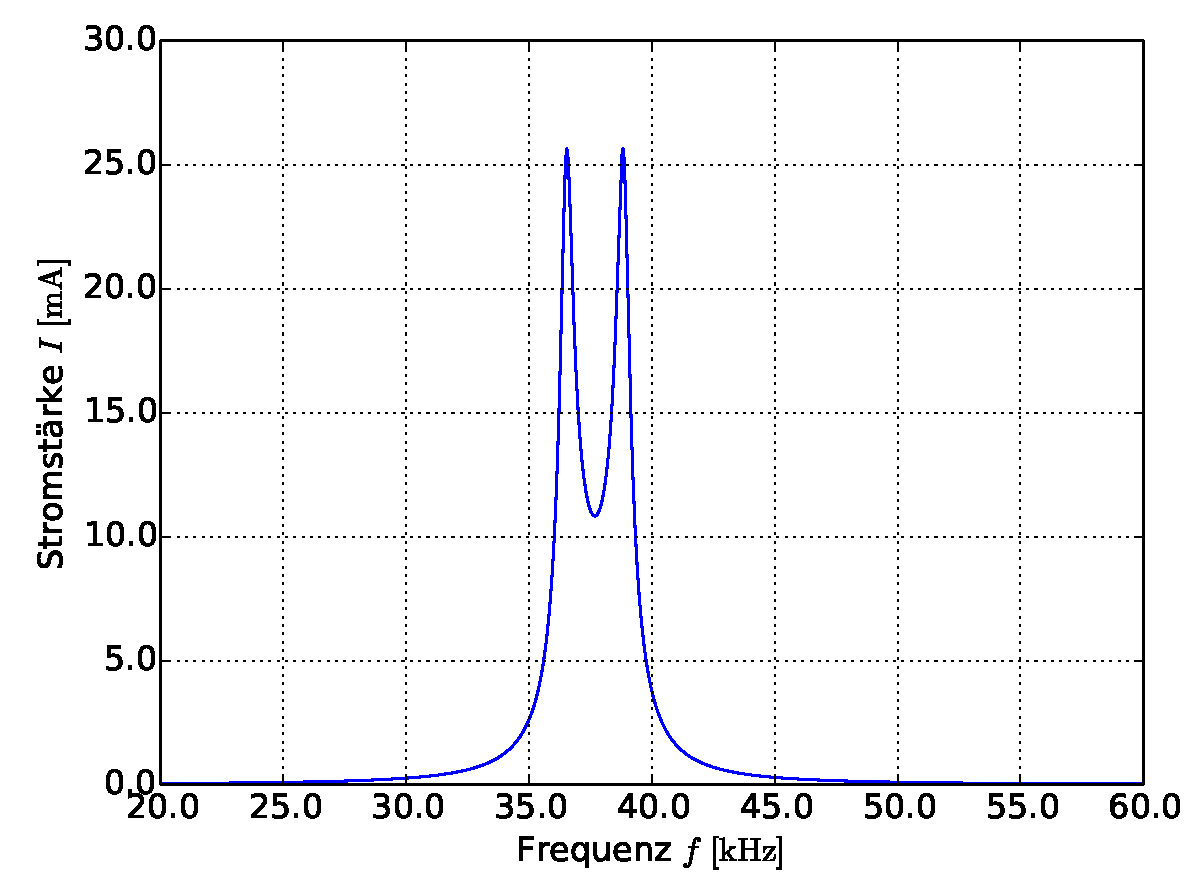
\includegraphics[scale=0.4]{Grafiken/Stromverlauf7.pdf}}
		\caption{Stromverläufe unter Verwendung verschiedener Koppelkondensatoren $C_{K}$}
		\label{fig:Auswertung_I2_Theo}
\end{figure}
	
	